\documentclass[a4paper,10pt]{article}
\usepackage[utf8x]{inputenc}
\usepackage{amsmath}
\usepackage{amsfonts}
\usepackage{relsize}
\usepackage[smaller]{acronym}
\usepackage{graphicx}
\usepackage{subfigure}
\usepackage{cite}
\usepackage{url}
\usepackage{hyperref}
\usepackage{color}
\usepackage[version=3]{mhchem}

\usepackage[left=3cm,right=3cm,top=3cm,bottom=3cm]{geometry}

\acrodef{WSN}{Wireless sensor network}
\acrodef{TEG}{Thermoelectric generator}
\acrodef{EH}{Energy harvesting}
\acrodef{PZT}{lead zirconate titanate}

%opening
\title{Energy Harvesting}
\author{Author: Miha \v Can\v cula \\ Mentor: doc. dr. Du\v san Ponikvar}

\begin{document}

\maketitle

\tableofcontents

\section{Introduction}

Small electronic devices are increasingly present everywhere around us. With their ubiquity and ever decreasing size and power consumption, connecting each of them to the power grid becomes impractical. 

The traditional solution is to use batteries, but they come with their own set of problems. Replacing them can be expensive, especially in hard-to-reach places. A much better option would be if the device had a power source of its own, removing its dependence on the power grid and drastically reducing the maintanace cost~\cite{Burgoine11}. 

The practice of drawing small amounts of electricity from the device's immediate surrounding is called \ac{EH}. 

\section{Use-cases and requirements}

\subsection{Sensors}

A very common useBoth the output voltage and the source resistance are directly proportional to the number of couples in the series, so it is important to use the right size of the generator to ensure a high enough voltage while still keeping the resistance low~\cite{Salerno10}. Characteristics of one example generator are given in Table~\ref{tab:teg-radiator}. Mounted on a radiator with temperature 30 K higher than that of the surrounding air, four such generators stacked in layers are is capable of producing 60 mW of power at 700 mV~\cite{teg-wsn-ieee}. 

 for energy harvesting systems are nodes in \acp{WSN}~\cite{teg-wsn-ieee,cap-wsn-ieee}. Such a network can contain a large number of independent nodes, so it would be difficult to connect each node to the power grid with wires. The sensors themselves usually consume very small amounts of power, so they are ideal applications for \acl{EH} methods. 

% list is from wikipedia: https://en.wikipedia.org/wiki/Energy_harvesting
The applications for \acp{WSN} include~\cite{wiki:eh}:
\begin{itemize}
  \item Weather stations
  \item Air and water pollution measuring
  \item Fire detection
  \item Industrial machine health monitoring
  \item Structural monitoring in buildings
  \item Intelligent buildings~\cite{cap-wsn-ieee}
\end{itemize}

Most of these applications require the nodes to be outside or in other areas where a direct connection to the grid would be difficult. On the other hand, they can still be close enough to the central node so they can transmit the measurements over a wireless connection with their own harvested power. 

Another important characteristic of sensor nodes is their power consumption profile. Often they will be idle for a long time (from minutes to days), and perform measurements in a relatively short time. The transmission of data can be even more infrequent, depending on whether the data has to be available immediately or not. In any case, sensor nodes consume very little current in the idle time period, with short bursts of consumption at regular intervals. An example of such consumption profile in is Figure~\ref{fig:wsn-consumption}. 

\begin{figure}[h]
\centering
 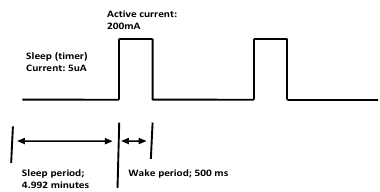
\includegraphics[width=250pt]{./Slike/wsn-current-profile}
 \caption{An example of a \ac{WSN} current consumption profile~\cite{cap-wsn-ieee}}
\label{fig:wsn-consumption}
\end{figure}

The average power consumption depends mostly on the duty cycle. If the measurement and especially the transmission of data does not have to be very frequent, the average consumption can be made very low. The consumption during the inactive time is often of the order of a few $\mu W$~\cite{Salerno10}. For example, electrical characteristic of an automatic radiator valve which take a measurement every hour are listed in Table~\ref{tab:zbarv}. This system draws an average power of 1 mW and would normally need it batteries changes at least once a year~\cite{teg-wsn-ieee}. 

\begin{table}[h]
  \centering
  \begin{tabular}{|c|c|}
\hline
    Parameter & Value \\
\hline
Supply Voltage & 2.7 - 3.3V \\
Working current & 60 mA \\
Sleeping current & 10 $\mu$A \\
Working duration & 20 seconds/hour \\
Working duration & 3579 seconds/hour \\
\hline
  \end{tabular}
\caption{Electrical characteristics of an automated radiator valve}
\label{tab:zbarv}
\end{table}

\subsection{Consumer electronics}

Many popular electronic devices, including TV remote controls, digital watches, portable music players and mobile phones, have power consumption low enough to be powered or at least assisted by \ac{EH}. Although their batteries can last a very long time, they can run out unexpectedly and cause a severe inconvenience. 

Solar cells on pocket calculators are very common and well-known, but so far their use has not spread to other electronic devices. There are, however, studies and working examples of remote controls for television and cars using a piezoelectric generator powered by the pressing force of our fingers, so this might change in the near future. 

\section{Photovoltaic cells}

The best known method of generating electricity from the environment on a small scale are photovoltaic cells. In most environments, they provide the highest power output of all \ac{EH} devices. 

\subsection{Theory}

The solar cells work by using the photovoltaic effect to create electron-hole pairs in a two-layer semiconductor by exciting the electrons to the conduction band. Once in the conduction band, the electron moves to the n-doped side with lower potential without crossing the gap. The flow of electrons from one side of the cell to the other creates voltage between the two metal contacts~\cite{wiki:solar-cells}. A diagram of potential levels and the electron's path can be seen in Figure~\ref{fig:pv-band-diagram}. 

\begin{figure}[!h]
\centering
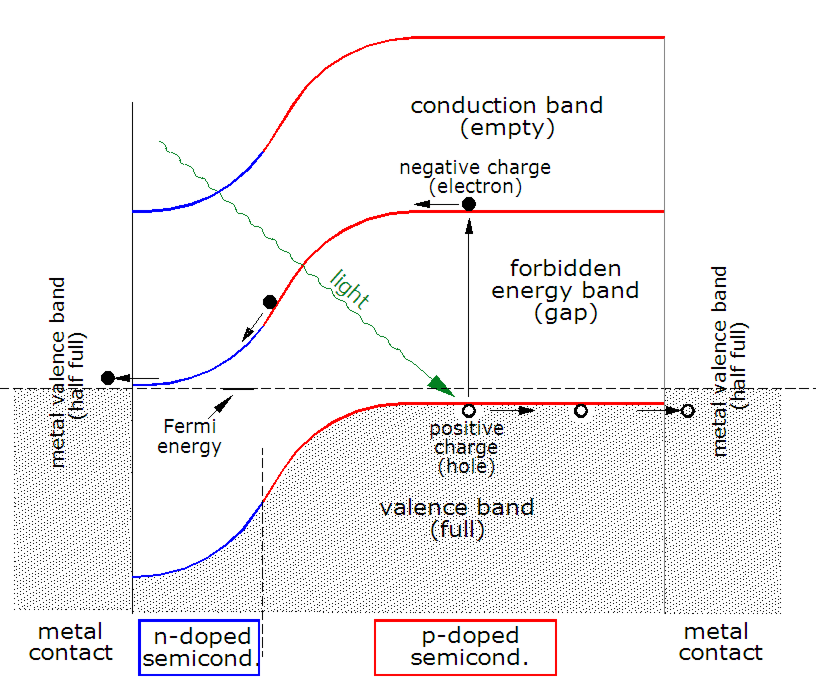
\includegraphics[width=0.7\textwidth]{./Slike/PV-band-diagram}
 \caption{Band diagram of a solar cell~\cite{wiki:solar-cells}}
\label{fig:pv-band-diagram}
\end{figure}

\subsection{Efficiency}

The downside of solar generators is the constant changing of their power output. Fortunately, there are several methods to work around this shortcoming. One way to is to use supercapacitors~\cite{cap-wsn-ieee} to store the produced energy. Even so, with variable weather conditions, the cell is not always operating with its peak efficiency. The shift in its optimal power point can be seen in Figure~\ref{fig:pv-power-curve}. It is possible to offset this by using a system that dynamically adjusts the cell voltage to find the maximum power point~\cite{solar-mppt-ieee}. 

\begin{figure}[h!]
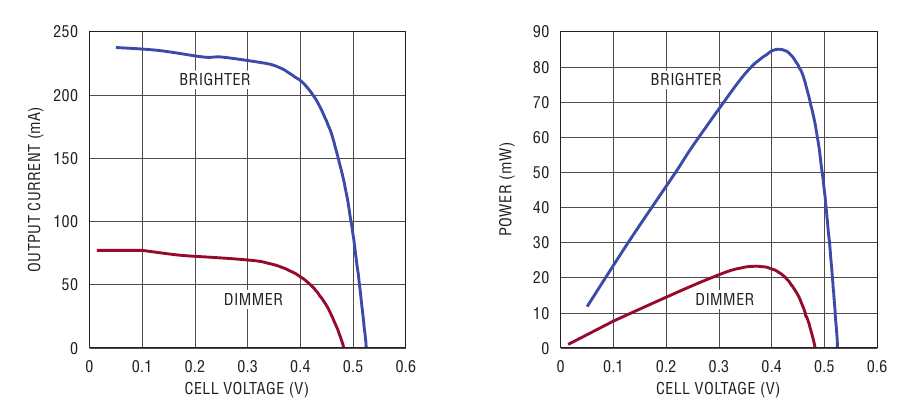
\includegraphics[width=\textwidth]{./Slike/PV-power-curve}
 \caption{Typical $I(V)$ and power curve of a 2x1 inch (13 cm$^2$) polycrystalline cell~\cite{Burgoine11}}
\label{fig:pv-power-curve}
\end{figure}

Modern photovoltaic cells can reach efficiencies up to 30\%. However, it is possible to use mirrors or lenses to concentrate more sunlight onto the cell, effectively raising it efficiency up to 45\%. This is useful because the concentrating optics are usually cheaper than solar cells themselves. On the other hand, such concentrators often require a system for tracking the sun, resulting in a more complicated solution, and are better suited for large-scale operations than for energy harvesting devices. 

\section{\acl{TEG}}

Another source of energy in the environment is a temperature gradient. Using the Seebeck effect, it is possible to convert this difference in temperatures into electricity. This method has become very popular in the recent years, mostly due to their reliability and lower cost than photovoltaics. The Seebeck effect is the converse of the better-known Peltier effect, so the same elements can be used for either thermoelectric cooling or power generation. 

\subsection{Construction}

\acp{TEG} are typically made from a series of alternating N-doped and P-doped semiconductors, sandwiched between two ceramic plates~\cite{Salerno10}. A schematic of their design can be seen in Figure~\ref{fig:teg-schematic}.

\begin{figure}[h]
\subfigure{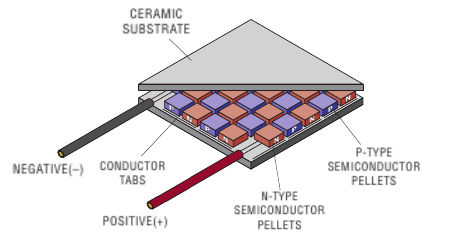
\includegraphics[height=100pt]{./Slike/TEG-shema}}
\subfigure{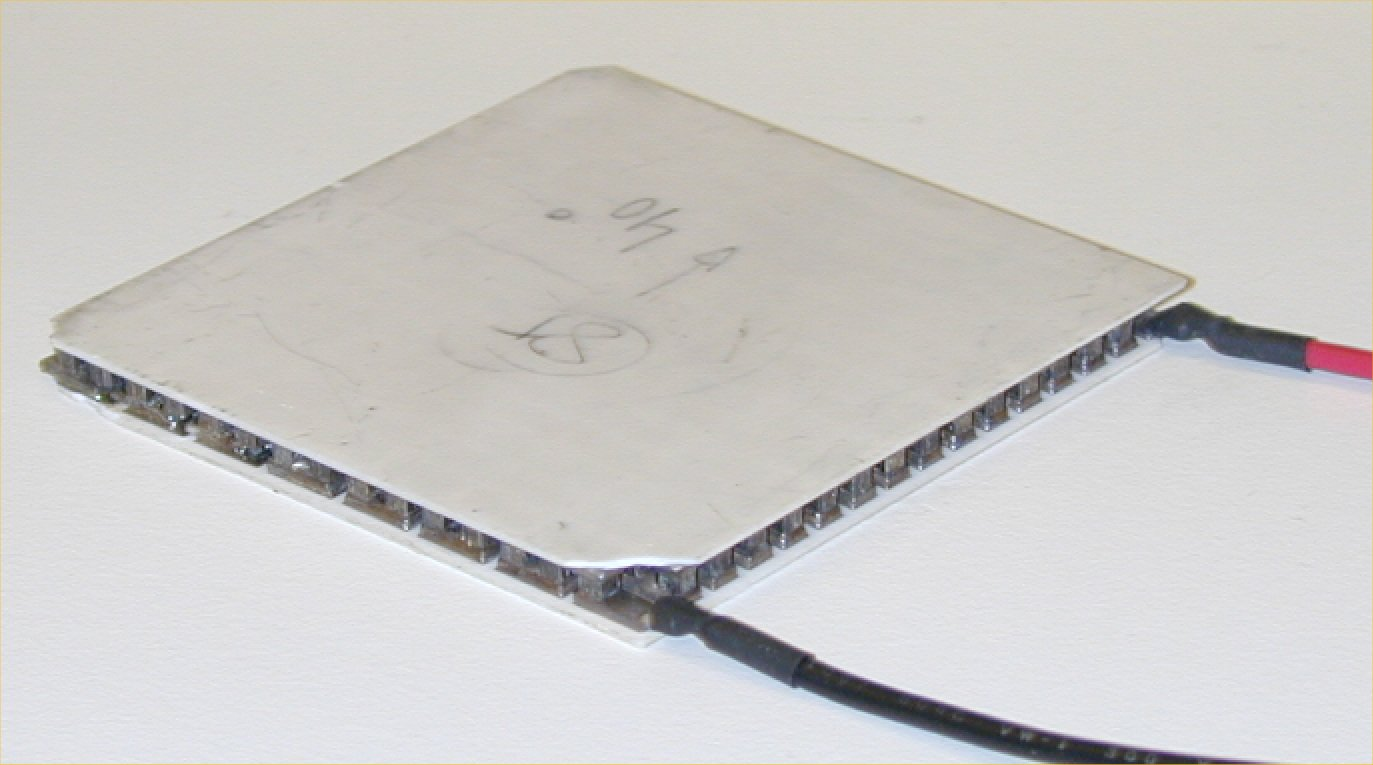
\includegraphics[height=100pt]{./Slike/TEG-slika}}
\caption{A schematic (left) and a photo (right) of a \ac{TEG} element~\cite{Salerno10,wiki:teg}}
\label{fig:teg-schematic}
\end{figure}

Due to their simple design and the possibility to re-use existing Peltier coolers, \ac{TEG} can be much cheaper than other \ac{EH} devices. 

\subsection{Characteristics}

Both the output voltage and the source resistance are directly proportional to the number of couples in the series, so it is important to use the right size of the generator to ensure a high enough voltage while still keeping the resistance low~\cite{Salerno10}. Characteristics of \texttt{TEC1-12709}, a common thermoelectric element which costs \$7.25, are given in Table~\ref{tab:teg-radiator}. Mounted on a radiator with temperature 30 K higher than that of the surrounding air, four such generators stacked in layers are capable of producing a maximum of 60 mW at 700 mV~\cite{teg-wsn-ieee}. 

\begin{table}[h]
  \centering
  \begin{tabular}{|c|c|}
\hline
    Parameter & Value \\
\hline
Dimensions & 30 x 34 x 3.2 mm \\
Maximum $\Delta T$ & 77 K \\
Number of couples & 127 \\
Device resistance & 3.78 $\Omega$ \\
\hline
  \end{tabular}
\caption{Physical properties of a \ac{TEG}}
\label{tab:teg-radiator}
\end{table}

\section{Piezoelectric generators}

The third most common form of \ac{EH} is generating power from the energy of motion. Vibrations are present especially in the vicinity of working machinery, but energy can also be produced from human activities, such as walking~\cite{piezo-shoe-ieee}. 

Certain clystalline materials with asymmetric unit cells polarize themselves when an external force is applied. This phenomenon is called the Piezoelectric effect. The best-known material to exhibit piezoelectric behavior is \ac{PZT}, a ceramic with the formula \ce{Pb[Zr_xTi_{1-x}]O3}, $0\leq x \leq 1$.

\subsection{Characteristics}

\begin{figure}[h!]
\centering
  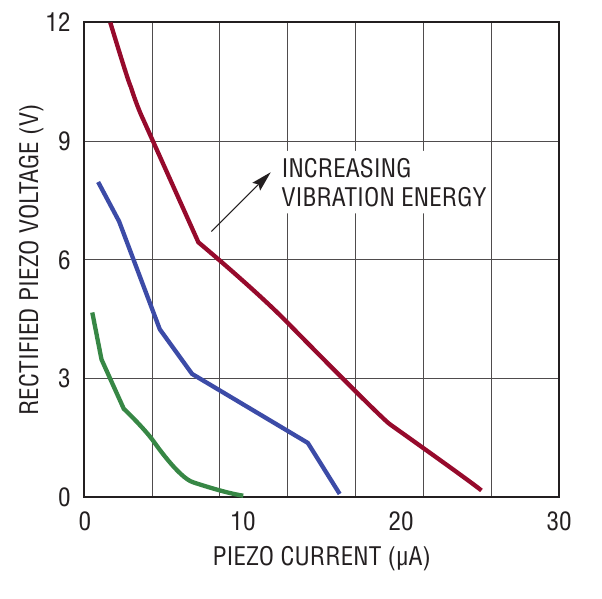
\includegraphics[width=0.5\textwidth]{./Slike/Piezo-UI}
\caption{Typical piezoelectric load lines~\cite{LT-Piezo}}
\label{fig:piezo-load}
\end{figure}

Unlike other \ac{EH} methods, piezoelectric elements often produce relatively high voltages, so a converter is needed to decrease the voltage. Both open-circuit voltage and short-circuit current increase with the available vibration energy~\cite{LT-Piezo}. Figure~\ref{fig:piezo-load} shows load lines for Piezo Systems \texttt{T220-A4-503X} rated for voltages up to $\pm$180 V with a wholesale price of \$70 per piece. In typical vibration energy harvesting applications, the output voltage is much lower, but still high enough to require a specialized power supply. 

Using a smaller device, researchers were able to produce produce an average power of over 8 mW from a \ac{PZT}-based piezoelectric mounted inside a shoe. This was enough to continuously power a short range radio frequency emitter~\cite{piezo-shoe-ieee}. 

% Ne vem ce je to fajn vkljucit, je uporabno ampak staro (2000)
% According to research by Volvo Car Company, a piezo-element with dimensions of 67 x 25 x 1.45 mm requires the user to press a button with a force of 10 N to generate enough energy to send a signal to the car. 

\section{Energy storage}

As mentioned above, electrical power from \ac{EH} generators can be very sporadic, and so can be the required load. Therefore, managing and storing the produced energy is very important. 

In most cases, energy is stored either in batteries or ultracapacitors. Ultracapacitors, also known as Electric double-layer capacitors, are the newer technology, and are used where higher power density (as opposed to energy density) is required. En example of such a system is a wireless sensor node with its short spike of power consumption during transmission of data~\cite{cap-wsn-ieee}. Other advantages of supercapacitors include long life with no danger of overcharging or over-discharging and low internal resistance, while their main disadvantages are lower energy density and high self-discharge rate~\cite{wiki:edlc}. 

\begin{figure}[!h]
\def\svgwidth{0.8\textwidth}
 \input{./Slike/Supercapacitors_chart.pdf_tex}
\caption{Comparison of energy storage options~\cite{wiki:edlc}}
% Sem vzel iz Wikipedije, morda bi bilo prav citirati
\label{fig:storage-chart}
\end{figure}

Obviously, the choice of the energy storage method depends on the applications. For a solar-powered calculator, batteries have an advantage because of their lower leakage, and the device never requires a power output. It is also possible to use both, an ultracapacitor for sudden spikes and a battery for long-term energy storage. 

\section{Conclusion}

\acf{EH} is becoming increasingly viable as a power source for small electronic devices. Because of their remote location or simply due to their small size and large numbers, it may become impractical or even impossible to connect such devices to the power grid or to supply them with batteries. Hence, an included small power source can drastically simplify the device installation and reduce its maintanace costs. 

We have seen three different methods for drawing power from the device surrounding, provided we have a source of light, heat or motion. The choice of a suitable method obviously depends on the device and the environment in which it is meant to be used. There are other possible approaches, but these three are the most popular at this time. 

Because the energy source might not be present at all times, as is the case with photovoltaic placed outdoors, we also need to store the harvested energy. In this field, ultracapacitors are seeing rapid development and have become an alternative to more traditional batteries. Many wireless devices have a short duty cycle, during which the higher power output of capacitors is an important advantage, while their average power consumption is still very low. 

\bibliography{harvesting}
\bibliographystyle{unsrt} 

\end{document}
